\begin{sol}
\begin{enumerate}[label=\textbf{(\alph*)}]
\item
Let $P$ is power output of the sun. The power reaches to sail is $P\frac{A}{4\pi r^2}$ where $r$ is distance between sail and sun.
Let $\dd N$ number of photons that collide with sail with time $\dd t$. We can write following formula $P\frac{A}{4\pi r^2}\dd t=\dd N E$, where $E$ is energy of a photon. The energy of a photon is $E=pc$ , $p$ is momentum.
So we can find total impulse that photons give to sail. The total momentum change will be $2\dd Np$ since sail is refractive. The total momentum will be $2P\frac{A}{4\pi r^2c}\dd t$. So $F=\dv{p}{t}$, force exerted on sail will be $F=2P\frac{A}{4\pi r^2c}$. And if we set this equal to
gravitational force we will get maximum area density: $$2P\frac{A}{4\pi \cancel{r^2}c}=\frac{GMm}{\cancel{r^2}}$$ and area density is $$\sigma=\frac{P}{2\pi GM}$$
\item
The maximum area density is different this time because there's absorbtion instead of reflection. The force balance will be $$\frac{P\pi R^2}{4\pi r^2c}=\frac{GM\sigma_{max}4\pi R^2}{r^2}$$ and our shell's is 
$\sigma=\frac{\sigma_{max}}{2}=\frac{P}{32\pi GMc}$. Coming to actual situation if we write work energy theorem $$\int_0^\infty \qty(\frac{P\pi R^2}{4\pi r^2c}-\frac{GMm}{r^2})\dd r=\frac{mv^2}{2}$$ and substituting what we got earlier we
get $$\int_0^\infty\frac{GMm}{r^2}\dd r=\frac12mv^2$$ evaluating integral gives us $\frac{GMm}{r}$ and our final speed is $$v=\sqrt{\frac{2GM}{r}}\approx 42124.18 m/s$$
\item here is a solution with picture(we couldn't compile it within the time)
\newline
\newline
\begin{center}
    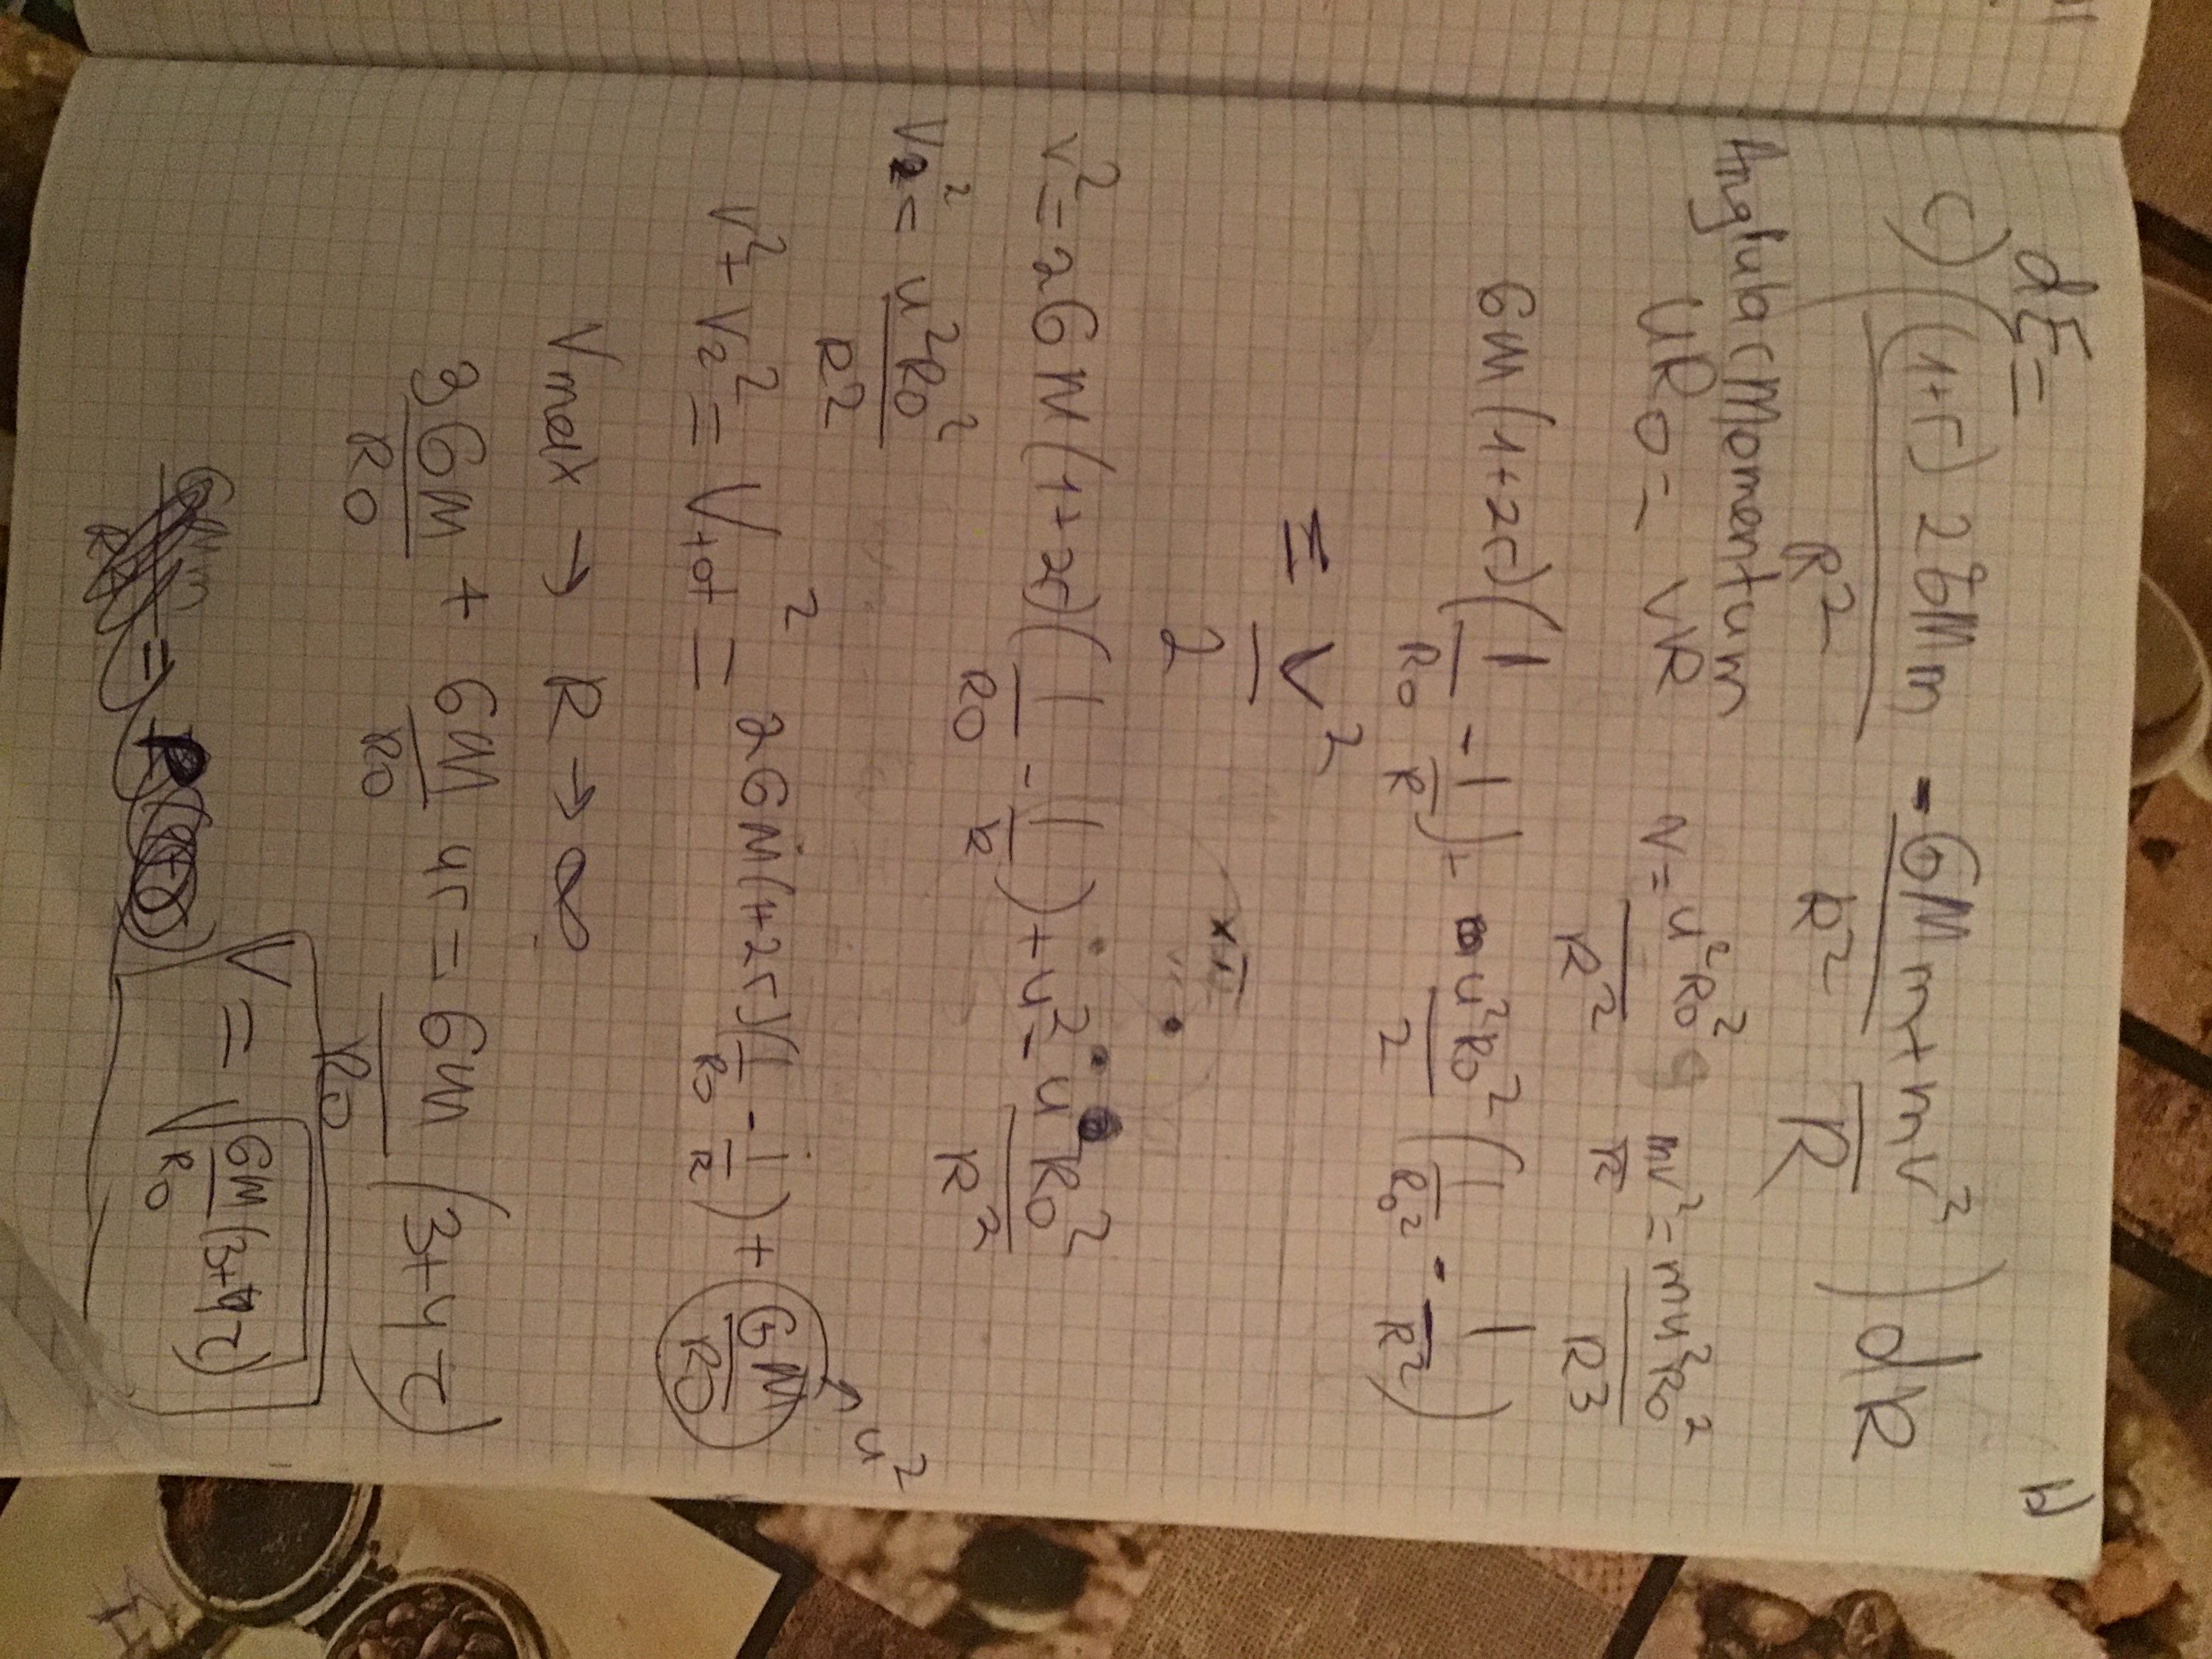
\includegraphics[width=\columnwidth, angle=90]{question2_partC.jpg}
\end{center}
\item
We assume that the laser is so powerful, its power does not change due distance from laser. So we can write work energy theorem for the  sail and then differentiate it. $$\gamma mc^2- \frac{P}{c}(1+r)x=const$$ differentiating it we get $\gamma^3m\dv{v}{t}=\frac{P}{c}(1+r)$. So seperating variables we get :
$$\int_0^{0.2c}\frac{m}{\qty(1-\frac{v^2}{c^2})^{3/2}}\dd v=\int_0^t\frac{P}{c}(1+r)\dd t$$ we can integrate it by substituting $\frac{v}{c}=\sin\theta$. We get 
$$mc\frac{\tfrac{v}{c}}{\sqrt{1-\tfrac{v^2}{c^2}}}\eval_0^{0.2c}=\frac{P}{c}(1+r)t$$
So power of the laser is $P=\frac{mc^20.2}{\sqrt{1-0.2^2}(1+r)t}$
\item
\end{enumerate}
\vspace{15mm}
\end{sol}